\chapter{Phương pháp đề xuất}

\section{Áp dụng mô hình WordGCN vào mô hình Transformer}

Ở mô hình đề xuất, sinh viên muốn thay thể module mã hóa \textit{embedding} đầu vào và cả mã hóa \textit{embedding} đầu ra bằng các \textit{embedding} được huấn luyện thuông qua mô hình \textit{WordGCN}.

Ở mô hình đề xuất \textit{Transformer} \cite{transformer}, lớp mã hóa embedding đầu vào và đầu ra được cài đặt bằng một lớp feed forward. Ban đầu, các token được mã hóa bằng phương pháp \textit{onehot encoding}. Sau đó, được mã hóa thành các embedding của kích thước d = 512. 
Gọi $W$ có kích thước $n_{voc} \times d$ là ma trận trọng số của lớp mã hóa embedding đầu vào và đầu ra. Với $n_{voc}$ là số lượng từ vựng trong kho ngữ liệu và $d$ là số chiều của embedding. Embedding tương ứng với từ thứ i trong kho ngữ liệu được tính bằng công thức:
\begin{equation*}
	e_x = i_x \times W
\end{equation*}

Trong đó, $e_x$ là \textit{embedding} của từ thứ x còn $i_x$ là \textit{vector one-hot encoding} của từ thứ x.

\begin{figure}[H]
    \begin{center}
        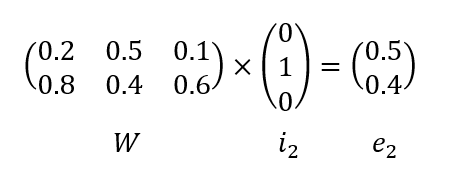
\includegraphics[scale=0.8]{images/original_input_embedding}
        \caption{Minh họa lớp mã hóa embedding với số lượng từ vựng trong kho ngữ liệu $n_{voc} = 3$ và số chiều của embedding $d = 2$}
        \label{fig:original-input-embedding}
    \end{center}
\end{figure}

Các tiếp cận này chưa khai thác được các đặc trưng về cú pháp và các đặc trưng về ngữ nghĩa của các từ vựng trong một ngôn ngữ. Bằng cách sử dụng WordGCN, các embeddings sẽ được huấn luyện trước qua 2 mô hình \textit{SynGCN} và \textit{SemGCN}. Kết quả sẽ được lưu vào trong một tập tin. Sau đó được truyền truyền thẳng vào mô hình  \textit{transformer} .

(Hình minh họa quá trình)

\section{Chuẩn bị dữ liệu}

\subsection{Tập dữ liệu WMT14}
\textit{WMT14 (Workshop on Statistical Machine Translation 2014)} \cite{wmt14} là một workshop chia sẻ về các bài toán được quan tâm trong lĩnh vự dịch máy. Trong đó, có 4 bài toán:
\begin{itemize}
	\item Translation task 
	\item Quality estimation task 
	\item metric task 
	\item Medical translation task
\end{itemize}

Trong phạm vi của khóa luận, sinh viên quan tâm đến bài toán dịch máy (translation task) với 2 ngôn ngữ là tiếng Anh và tiếng Đức. 

Với tập dữ liệu huấn luyện, WMT14 đã cung cấp khoảng 4.5 triệu câu từ 3 kho ngữ liệu song ngữ Anh-Đức:
\begin{itemize}
	\item Kho ngữ liệu song ngữ \textit{Europarl}: Được trích xuất từ các thủ tục hành chính của nghị viện Châu Âu
	\item Kho ngữ liệu song ngữ \textit{News Commentary}: bao gồm bình luận chính trị và kinh tế được thu thập từ trang web Project Syndicate
	\item Kho ngữ liệu song ngữ \textit{Common Crawl}: bao gồm các thông tin được thu thập từ tổng hợp các nguồn trên internet.
\end{itemize}

Với tập dữ liệu kiểm thử, dữ liệu được tổng hợp từ các mẫu truyện từ internet. Theo \cite{wmt14}, tập kiểm thử bao gồm 1500 câu tiếng Anh được dịch sang tiếng Đức và 1500 câu tiếng Đức được dịch về tiếng anh. Các mẫu dịch được cung cấp bởi các chuyên gia từ \textit{Capita}. 

\begin{table}[H]
	\centering
    \caption{Bảng thống kê số liệu của kho ngữ liệu song ngữ \textit{Europarl}}
    \label{tab:Europarl}
	\begin{tabular}{l|cc|}
	\cline{2-3}
		& \multicolumn{2}{c|}{\textbf{German $\leftrightarrow$ English}} \\ \hline
		\multicolumn{1}{|l|}{\textbf{Sentences}} & \multicolumn{2}{c|}{1,920,209} \\ \hline
		\multicolumn{1}{|l|}{\textbf{Words}}          & \multicolumn{1}{c|}{50,486,398} & 53,008,851 \\ \hline
		\multicolumn{1}{|l|}{\textbf{Distinct words}} & \multicolumn{1}{c|}{381,583} & 115,966 \\ \hline
	\end{tabular}
\end{table}

\begin{table}[H]
	\centering
	\centering
    \caption{Bảng thống kê số liệu của kho ngữ liệu song ngữ \textit{New Commentary}}
   \caption{}
    \label{tab:New Commentary}
	\begin{tabular}{l|cc|}
		\cline{2-3}
		& \multicolumn{2}{c|}{\textbf{German $\leftrightarrow$ English}} \\ \hline
		\multicolumn{1}{|l|}{\textbf{Sentences}}      & \multicolumn{2}{c|}{201,288}                  \\ \hline
		\multicolumn{1}{|l|}{\textbf{Words}}          & \multicolumn{1}{c|}{5,105,101}   & 5,046,157  \\ \hline
		\multicolumn{1}{|l|}{\textbf{Distinct words}} & \multicolumn{1}{c|}{150,760}     & 65,520     \\ \hline
	\end{tabular}
\end{table}

\begin{table}[H]
	\centering
    \caption{Bảng thống kê số liệu của kho ngữ liệu song ngữ \textit{Common Crawl}}
    \label{tab:Common Crawl}
	\begin{tabular}{l|cc|}
	\cline{2-3}
	& \multicolumn{2}{c|}{\textbf{German $\leftrightarrow$ English}} \\ \hline
	\multicolumn{1}{|l|}{\textbf{Sentences}}      & \multicolumn{2}{c|}{2,399,123}               \\ \hline
	\multicolumn{1}{|l|}{\textbf{Words}}          & \multicolumn{1}{c|}{54,575,405} & 58,870,638 \\ \hline
	\multicolumn{1}{|l|}{\textbf{Distinct words}} & \multicolumn{1}{c|}{1,640,835}  & 823,480    \\ \hline
	\end{tabular}
\end{table}

\subsection{Tiền xử lý dữ liệu cho mô hình SynGCN}

\subsubsection{Định dạng của dữ liệu}

Theo \cite{github.wordgcn}, dữ liệu đầu vào của \textit{SynGCN} phải được tiền xử lý thành các tập tin có cấu trúc như sau:
\begin{itemize}
	\item \textit{voc2id.txt}: Gán id cho mỗi từ trong kho từ vựng
	\begin{equation*}
		voc2id: W \rightarrow \mathbb{R}
	\end{equation*}
	\item \textit{id2freq.txt}: Thống kê tần số xuất hiện của các từ vựng không kho ngữ liệu
	\item \textit{de2id.txt}: Gán id cho các mối quan hệ trong universal dependencies
	\item \textit{data.txt}: Biểu diễn lại kho ngữ liệu theo định dạng:
	\begin{equation*}
	N\ M\ tok_1\ tok_2\ tok_3 ... tok_N\ dep_1\ dep_2 .... dep_M
	\end{equation*}
	\begin{itemize}
		\item N là số lượng từ trong câu và M là số lượng mối quan hệ giữa các từ trong câu.
		\item $tok_i$ là id của từ thứ i trong câu.
		\item $dep_i$ là mối quan hệ thứ i trong câu. Mỗi mối quan hệ được biểu diễn dưới dạng:
		\begin{equation*}
			source\_token|destination\_token|dep\_rel\_label
		\end{equation*}
		Trong đó, \textit{source\_token} và \textit{destination\_token} là hai từ phát sinh mối quan hệ với nhau. \textit{dep\_rel\_label} là mối quan hệ giữa hai từ này.
	\end{itemize}
\end{itemize}

\subsubsection{Voc2id}

WMT14 đã cung cấp sẵn cho ta tập V là tập hợp các từ vựng trong kho ngữ liệu. Do đó, ta chỉ cần đánh số thứ tự cho các từ trong V.

\begin{algorithm}[H]
    \caption{Tiền xử lý dữ liệu voc2id}
    \begin{algorithmic}[1]
		\State Khởi tạo $tok_{<unk>} = 0$
		\State Khởi tạo $count \gets 1$
		\For{$w \in V$}
			\State $tok_{w} = count$
			\State $count \gets count + 1$
		\EndFor
    \end{algorithmic}
\end{algorithm}

\subsubsection{id2freq}

\begin{algorithm}[H]
    \caption{Tiền xử lý dữ liệu id2freq}
    \begin{algorithmic}[1]
		\State Khởi tạo $\forall w \in V : freq_w = 0$
		\State Khởi tạo $freq_{<unk>} = 0$
		\For{$w \in W$}
			\If{$w \in V$} 
				\State $freq_{w} \gets freq_{w} + 1$
			\Else 
				\State $freq_{<unk>} \gets freq_{<unk>} + 1$
			\EndIf
		\EndFor
    \end{algorithmic}
\end{algorithm}

Trong đó, \textit{<unk>} là các từ lạ không nhận diện được từ bộ từ vựng.

\subsubsection{de2id}

Tập các mối quan hệ $Dep$ được tổng hợp từ \textit{Universal dependencies}.

\begin{algorithm}[H]
    \caption{Tiền xử lý dữ liệu de2id}
    \begin{algorithmic}[1]
		\For{$relation \in Dep$}
			\State $dep_{relation} = count$
			\State $count \gets count + 1$
		\EndFor
    \end{algorithmic}
\end{algorithm}

\subsubsection{data}

Theo \textit{WordGCN}, để có thể rút trích các mối quan hệ của các từ trong câu, ta sử dụng công cụ \textit{CoreNLP Parser}. Ở bước này, do các câu có thể xử lý một các độc lập nhau. Ta có thể chia tập dữ liệu ra thành các tập nhỏ hơn để xử lý giúp tăng hiệu quả tính toán và giảm gánh nặng tài nguyên. Các phần cứng chạy song song sẽ chia sẻ với nhau chung các tập tin \textit{voc2id}, và \textit{de2id}. Mỗi máy thành phần thứ $i$ sẽ được xử lý tập $S_i \subset S$ với $S$ là tập tất cả các câu trong kho ngữ liệu.


\begin{algorithm}[H]
    \caption{Tiền xử lý dữ liệu data}
    \begin{algorithmic}[1]
		\State $document = CoreNLP\_Parser(S_i)$
		\For{$sentence \in document$}
			\State Ghi số lượng từ trong câu vào data.txt
			\State Ghi số lượng quan hệ trong câu vào data.tx
			\For{$word \in sentence$}
				\If{$word \in V$}
					\State Ghi $tok_{word}$ vào data.txt
				\Else
					\State Ghi $tok_{<unk>}$ vào data.txt
				\EndIf
			\EndFor

			\For{$dep \in dependencies(sentence)$}
				\State Ghi $dep_{src}|dep_{dest}|dep_{relation}$ vào data.txt
			\EndFor
			
			\State Writeln
		\EndFor
    \end{algorithmic}
\end{algorithm}

\subsection{Tiền xử lý dữ liệu cho mô hình SemGCN}

\subsubsection{WordNet}

WordNet là kho ngữ liệu từ vựng gom nhóm các từ tương đồng thành các tập gọi là các synsets. Các từ trong một synset có thể được thay đổi cho nhau mà không làm thay đổi ý nghĩa của câu ở một số trường hợp nhất định.

Các mối quan hệ được đề cập trong WordNet chủ yếu là thượng-hạ vị. Ngoài ra còn cung cấp thêm các cặp từ trái nghĩa.

Khái niệm hạ vị chỉ một từ hoặc một cụm từ có ngữ nghĩa được kế thừa từ một từ khác. Từ đó, ta có khái niệm thượng vị là một từ có ngữ nghĩa chứa đựng ngữ nghĩa của một từ khác. Có thể thấy, thượng \- hạ vị là các mối quan hệ không đối xứng, và không thể có một từ vừa là thượng vị cũng vừa là hạ vị của một từ. Từ đó, ta có thể tạo ra được một rừng (tập hợp của các đồ thị con dạng cây) có hướng. Với các đỉnh cha là thượng vị của các đỉnh con.

Ngoài ra, ta còn có khái niệm đồng hạ vị (co-hyponym) chỉ các cặp từ cùng là hạ vị của một từ.

\begin{figure}[H]
    \begin{center}
        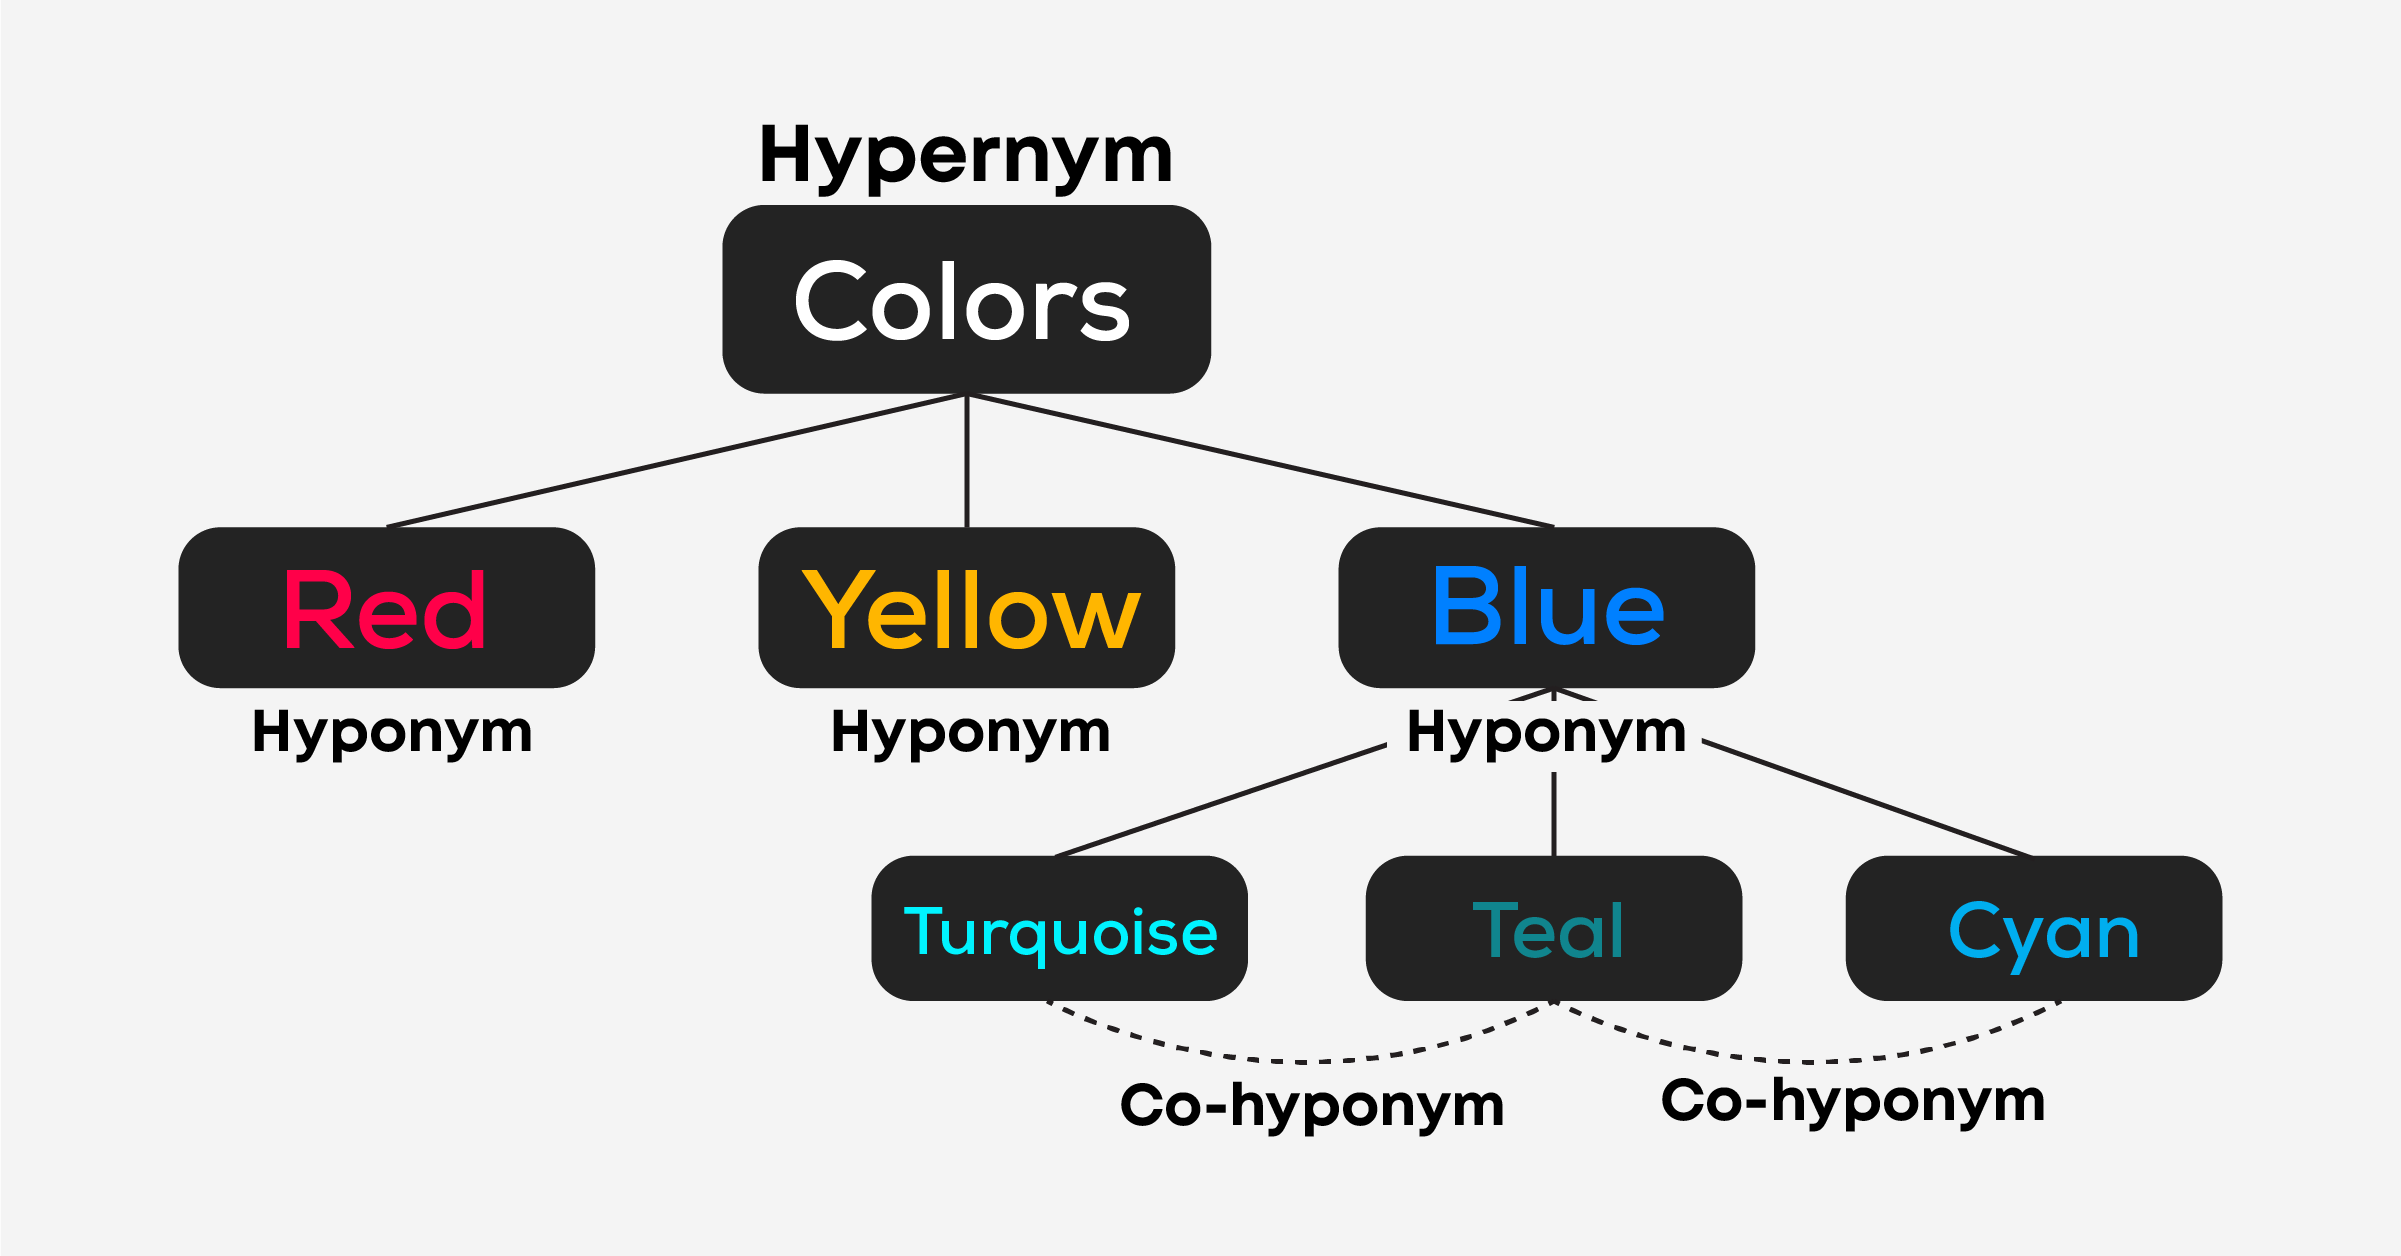
\includegraphics[scale=0.185]{images/hypernym-hyponym}
        \caption{Ảnh minh họa thượng vị và hạ vị}
        \label{fig:hypernym-hyponym}
    \end{center}
\end{figure}

Theo như ví dụ trên, các màu sắc "red" (đỏ), "yellow" (vàng) và "blue" (xanh dương) là các hạ vị của "colors" (màu sắc) do chúng đều có ý nghĩa là một màu sắc. "Colors" được gọi là thượng vị của "red", "yellow" và "blue". Bên cạnh đó, "yellow" và "blue" do có chung một thượng vị nên chúng được gọi là đồng thượng vị.


\subsubsection{Định dạng dữ liệu}

Theo \cite{github.wordgcn}, \textit{SemGCN} quan tâm đến 4 mối quan hệ ngữ nghĩa và được xác định bởi 4 tập tin sau:
\begin{itemize}
	\item \textit{Antonyms}: bao gồm các cặp từ có ý nghĩa trái ngược nhau trong kho từ vựng. Mối quan hệ trái nghĩa là mối quan hệ 2 chiều và sẽ biểu diễn bằng 2 cạnh đối nhau trong đồ thị ngữ nghĩa.
	\item \textit{Hypernyms}: chứa các cặp bao gồm một từ và thượng vị của nó. Mối quan hệ này là mối quan hệ một chiều.
	\item \textit{Hyponyms}: chứa các cặp từ bao gồm một từ và một hạ vị của nó. Mối quan hệ này cũng là moios quan hệ một chiều.
	\item \textit{Synonyms}: bao gồm nhiều dòng, với mỗi dòng biểu diễn một từ và tập các từ đồng nghĩa với từ đó.
\end{itemize}

Dựa trên \textit{WordGCN}, các mối quan hệ \textit{antonyms, hypernym} và \textit{hyponym} được trích xuất nhờ vào WordNet, còn mối quan hệ \textit{synonym} thì được trích xuất dựa vào PPDB (The paraphrase database).

\subsection{Tiền xử lý dữ liệu cho mô hình transformer}

Dữ liệu đầu vào của \textit{transformer} bao gồm 2 phần:
\begin{itemize}
	\item kho ngữ liệu WMT14 bao gồm các cặp câu song ngữ Anh-Đức.
	\item Các embedding được huấn luyện bởi mô hình WordGCN
\end{itemize}

Với dữ liệu WMT14, ta cần thực hiện tokenization các từ trong kho ngữ liệu với id của các từ phải tương ứng với id trong tập tin voc2id.txt. Ngoài ra, ta phải bổ sung thêm ba token đặc biệt vào vào bộ từ vựng như sau:
\begin{itemize}
	\item \textit{<pad>}: Ma trận chứa dữ liệu đầu vào của  \textit{transformer}  có kích thước $n \times len\_max$. Trong đó n là số lượng câu còn $len\_max$ là kích thước của câu có chiều dài dài nhất trong kho ngữ liệu. Do đó, dẫn đến một số hàng của ma trận sẽ không có giá trị. Ta bổ sung thêm một token đặc biệt này vào để lắp đầy các vị trí đó. Embedding tương ứng với \textit{<pad>} sẽ được gán giá trị bằng với vector 0.
	\item \textit{<bos>}: Token này dùng để đánh dấu bắt đầu của một câu. Giá trị của Embedding tương ứng sẽ được gán là vector với toàn giá trị 1 ở mọi chiều.
	\item \textit{<eos>}: token này dùng để đánh dấu kết thúc của một câu. Giá trị của Embedding tương ứng sẽ được gán là vector với toàn giá trị -1 ở mọi chiều.
\end{itemize}

\begin{figure}[H]
    \begin{center}
        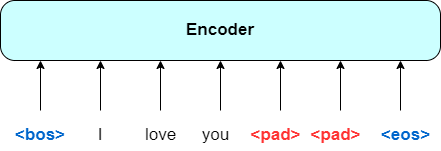
\includegraphics[scale=0.85]{images/special-token}
        \caption{Minh họa về các token đặc biệt trong mô hình \textit{transformer} }
        \label{fig:special token}
    \end{center}
\end{figure}

Dữ liệu các embedding đã được huấn luyện bởi mô hình WordGCN sẽ được lưu trữ trong một tập tin có dạng như sau:

\begin{figure}[H]
    \begin{center}
        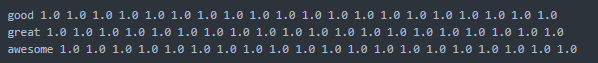
\includegraphics[scale=1]{images/pretrained-embedding}
        \caption{Định dạng của tập tin chứa các \textit{embedding} được huấn luyện bởi mô hình \textit{WordGCN}. Ở ví dụ này mỗi từ được biểu diễn bởi một embedding của số chiều là 20.}
        \label{fig:pretrained-embedding}
    \end{center}
\end{figure}

Mỗi dòng sẽ chứa thông tin về \textit{embedding} của một từ trong kho ngữ liệu. Trong đó:
\begin{itemize}
	\item Một từ đầu dòng thuộc kho ngữ liệu.
	\item $d$ số tiếp theo biểu thị giá trị của \textit{vector embedding} của từ đang xét.
\end{itemize}